
\documentclass[ms.tex]{subfiles} 
\begin{document} 

\section{The Multi-Zone Chemical Evolution Model} 
\label{sec:methods} 

\begin{figure*} 
\centering 
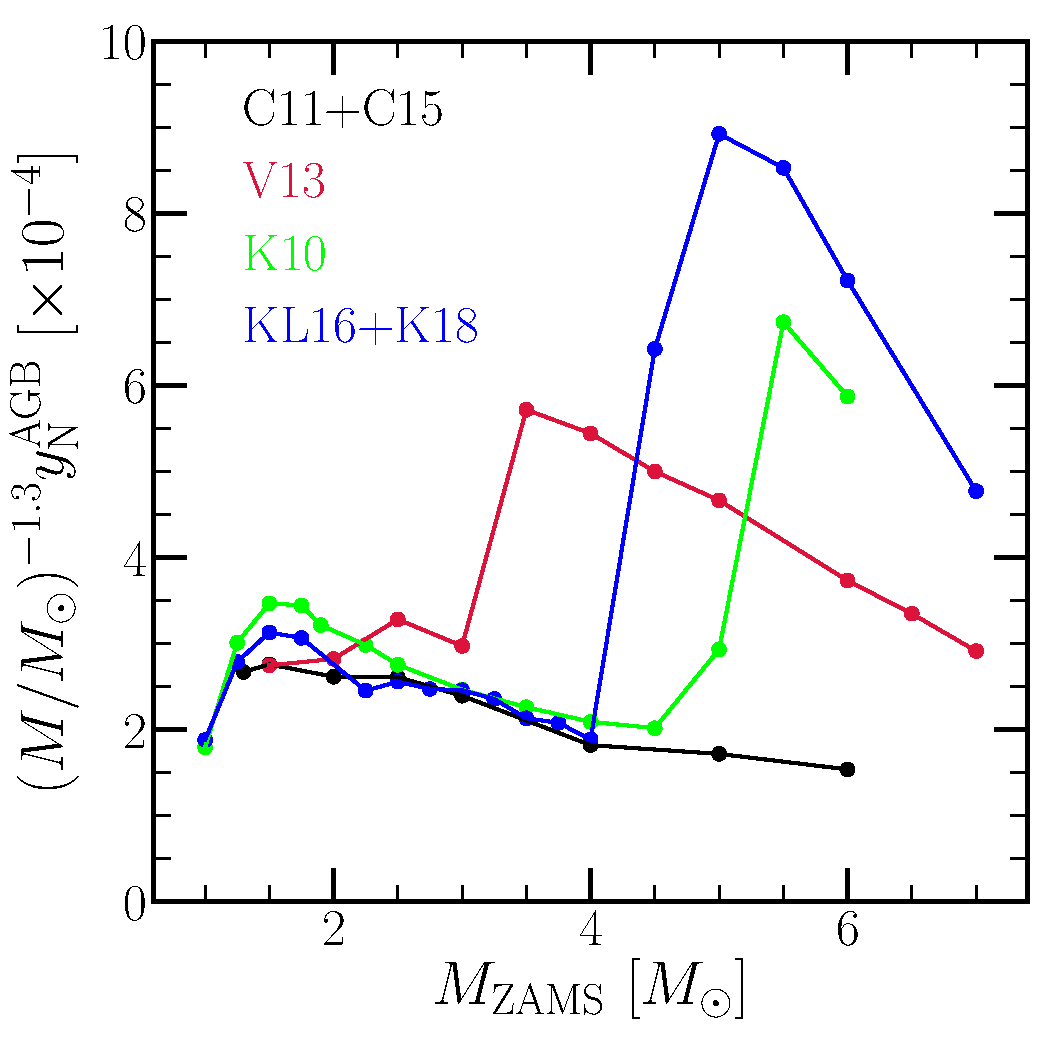
\includegraphics[scale = 0.3]{agb_yield_models_imfweighted.pdf} 
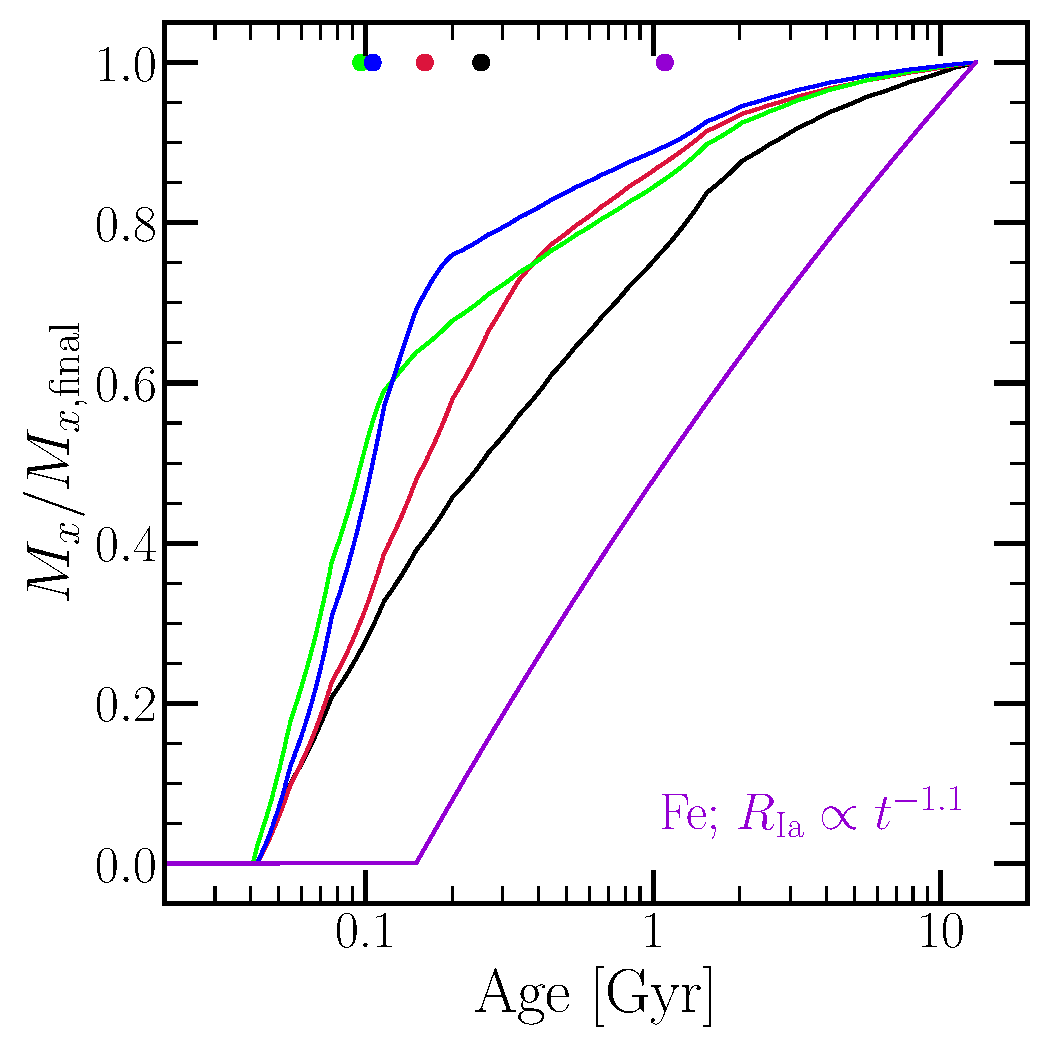
\includegraphics[scale = 0.3]{ssp_production_modelcomp.pdf} 
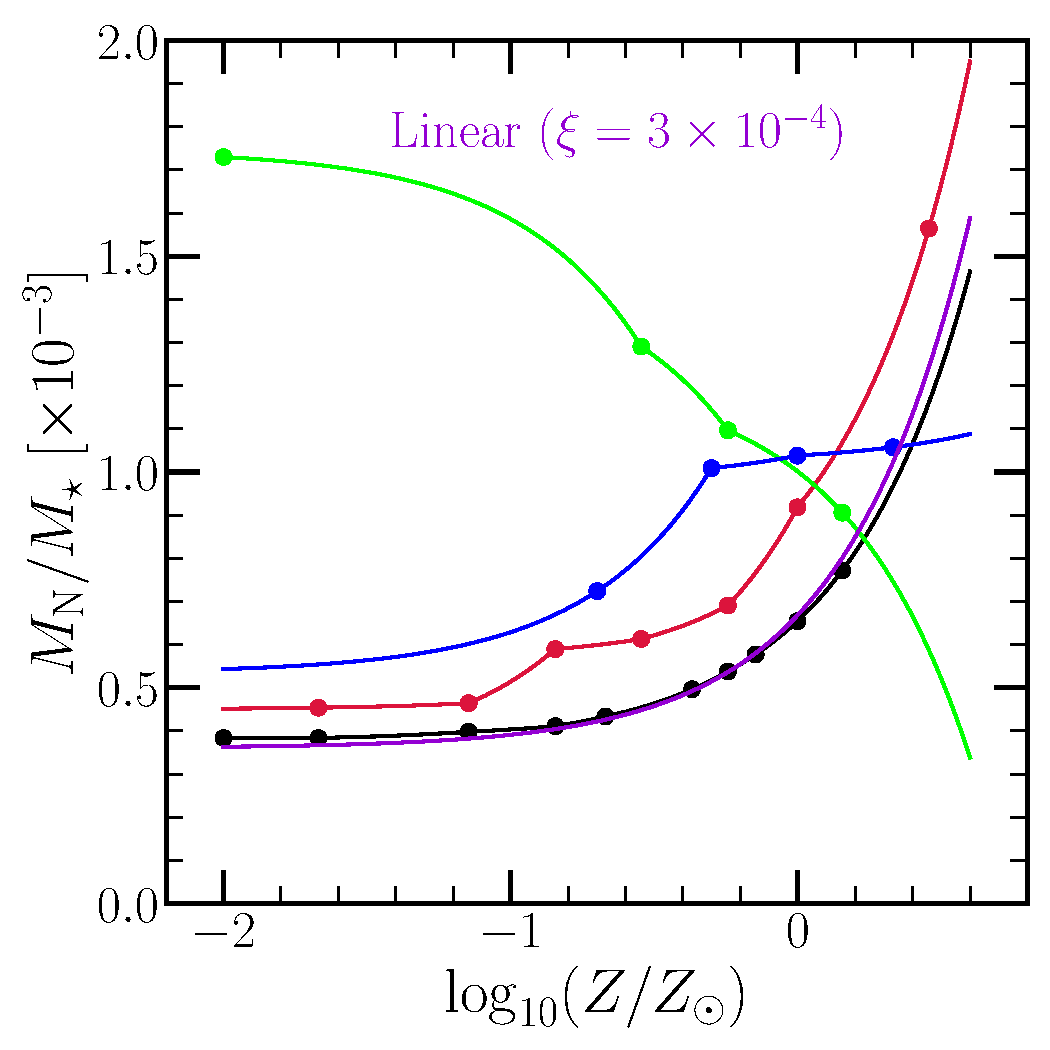
\includegraphics[scale = 0.3]{ssp_production_metdep.pdf} 
\caption{ 
\textbf{Left}: The IMF-weighted mass yield of N from AGB stars as a function 
of progenitor mass at solar metallicity ($Z = 0.02$ in~\karakasten,~$Z = 0.014$ 
otherwise). 
\textbf{Middle}: The net mass of N produced by AGB stars from a single stellar 
population for each of our yield models at the same metallicities as in the 
left panel. 
The purple line denotes the same for Fe assuming our~$t^{-1.1}$ delay time 
distribution. 
All values are normalized to the total mass produced at an age of 13.2 Gyr. 
Points at the top of the panel denote the ages at which 50\% of the total mass 
yield has been produced. 
\textbf{Right}: The total amount of N produced by a 13.2 Gyr old stellar 
population as a function of metallicity for each of our yield models normalized 
by the stellar population's initial mass. 
Points mark metallicities at which the published tables report yields. 
} 
\label{fig:ssp} 
\end{figure*} 

\begin{itemize} 
	\item Since we wish to test the impact of various assumptions about 
	nucleosynthetic yields while taking into account stellar migration, 
	multi-zone chemical evolution models are the ideal experiments. 
	This allows us not only to entertain different assumptions regarding 
	nucleosynthetic yields of N, but also affords us the ability to enforce a 
	specific star formation history as well as slight variations to any of 
	these assumptions - all within a framework that includes the impact of 
	radial migration. 

	\item We make use of the Milky Way models of~\citet{Johnson2021}, who 
	originally constructed the model to explore the impact of stellar migration 
	on the observed abundances of O and Fe. 
	This model makes use of the~\texttt{Versatile Integrator for Chemical 
	Evolution}~\citep[\vice;][]{Johnson2020, Griffith2021, Johnson2021}, an 
	open-source~\texttt{python} package for~\texttt{Unix} system architectures. 
	Because~\vice~recognizes most elements on the periodic table, computing 
	N abundances with this model is easy. 
	Though we provide a brief summary here, a full breakdown of 
	the~\citet{Johnson2021} model can be found in their~\S~2. 

	\item As in previous models for the Milky Way~\citep[e.g.][]{Matteucci1989, 
	Schoenrich2009, Minchev2013, Minchev2014, Minchev2017, Sharma2020}, this 
	model parameterizes the Galaxy disc as a series of concentric rings of 
	width~$\delta\rgal$ = 100 pc.
	Each ring is assigned its own star formation history (SFH), and with 
	assumptions about the~$\Sigma_\text{gas}-\dot{\Sigma}_\star$ relation and 
	outflows (see discussion below),~\vice~calculates the implied amounts of 
	gas and infall at each timestep automatically. 
	Each ring is assumed to be described by a conventional one-zone model of 
	chemical evolution under the caveat that stellar populations can move 
	between rings, which~\citet{Johnson2021} demonstrate has a significant 
	impact on the enrichment rates of delayed sources such as SNe Ia. 

	\item To drive stellar migration, the model makes use of star particles 
	from a hydrodynamical simulation, for which~\citet{Johnson2021} chose 
	the~\hsim~galaxy from the~\citet{Christensen2012} suite evolved with the 
	N-body+SPH code~\texttt{GASOLINE}~\citep{Wadsley2004}; we retain this 
	decision here. 
	Previous studies have shown that~\hsim, among other disc galaxies evolved 
	with similar physics, has a realistic rotation curve~\citep{Governato2012, 
	Christensen2014a, Christensen2014b}, stellar mass~\citep{Munshi2013}, 
	metallicity~\citep{Christensen2016}, dwarf satellite 
	population~\citep{Zolotov2012,Brooks2014}, HI properties~\citep{Brooks2017}, 
	and age-velocity relation~\citep{Bird2021}. 

	\item Despite this, there are some interesting differences 
	between~\hsim~and the Milky Way. 
	The last major merger in~\hsim~was at a redshift of~$z \approx$ 3, making 
	it an interesting case study for its quiescent merger 
	history~\citep[e.g.][]{Zolotov2012}. 
	The Milky Way is also known to have a strong, long-lived 
	bar~\citep[e.g.][]{Bovy2019}, while~\hsim~had only a weak and transient 
	bar, lacking one at the present day. 

	\item Radial migration proceeds from the~\hsim~star particles in a simple 
	manner; for a stellar population in our model born at a radius~\rgal~and a 
	time~$T$,~\vice~searches for star particles born at~$\rgal \pm$ 250 pc 
	and~$T \pm$ 250 Myr. 
	From the star particles that pass this cut, it then randomly selects one 
	to act as that stellar population's~\textit{analogue}. 
	The stellar population then assumes the present day midplane distance~$z$ 
	and the change in orbital radius~$\Delta\rgal$ of its analogue. 
	In the~\citet{Johnson2021} fiducial model, stellar populations move to 
	their implied final radii with a~$\sqrt{\text{age}}$ dependence, similar 
	to the assumption made by~\citet{Frankel2018, Frankel2019}. 
	While they investigate the impact of this assumption, in the present paper 
	we make use of only this model and one in which stellar migration is 
	ignored. 
	If~\vice~does not find any star particles from~\hsim~in its initial search, 
	it widens it to~$\rgal \pm$500 pc and~$T \pm$500 Myr; if still no 
	candidate analogues are found,~\vice~maintains the~$T \pm$500 Myr 
	requirement, but assigns the star particle with the smallest difference in 
	birth radius as the analogue. 
	As in~\citet{Johnson2021}, these models neglect the impact of radial 
	gas flows~\citep[e.g.][]{Lacey1985, Bilitewski2012, Vincenzo2020}, instead 
	focusing on the impact of stellar migration. 

	\item Although this model does impose some small but nonzero level of star 
	formation at early times in the outer disc, the sample of star particles 
	from~\hsim~is sufficiently large that stellar populations that form there 
	are typically assigned analogues which formed within~$\sim$2 kpc of their 
	birth radius. 
	While ignoring effects such as the radial growth of the Galaxy 
	(e.g.~\citealp*{Bird2012};~\citealp{Bird2013}), this at least ensures that 
	these old, outer disc populations are assigned stellar populations which 
	give them an outer disc rather than an inner disc dynamical history. 

	\item Rather than using a hydrodynamical simulation, some previous studies 
	have implemented stellar migration using dynamical 
	arguments~\citep[e.g.][]{Schoenrich2009, Sharma2020}. 
	\begin{itemize} 
		\item An advantage of our approach over this is that these dynamical 
		arguments introduce free parameters into the model which then require 
		fitting to data. 
		A disadvantage is that we are restricted to one realization of our 
		dynamical history; slight variations are not possible. 

		\item This model does not distinguish between ``blurring'' and 
		``churning'', terms often used to refer to a the epicyclic motions of 
		stars and changes in their guiding centres, respectively. 
		These effects are induced by a variety of physical interactions such as 
		molecular cloud scattering~\citep{Mihalas1981, Jenkins1990, 
		Jenkins1992}, orbital resonances with spiral arms or 
		bars~\citep{Sellwood2002, Minchev2011}, and satellite 
		perturbations~\citep{Bird2012}; both are present in~\hsim. 
	\end{itemize} 

	\item Our fiducial model here has the same SFH as that 
	of~\citet{Johnson2021}, where the time-dependence at a given~\rgal~is given 
	by: 
	\begin{equation} 
	f(t|\rgal) = (1 - e^{-t/\tau_\text{rise}})e^{-t/\tau_\text{sfh}}, 
	\end{equation} 
	where~$\tau_\text{rise}$ approximately controls the amount of time the SFR 
	is rising at early times; we set this parameter equal to 2 Gyr at all 
	radii as in~\citet{Johnson2021}. 
	Our e-folding timescales~$\tau_\text{sfh}$ are taken from a fit of this 
	functional form to the~$\Sigma_\star$-age relation in bins of~$R/R_\text{e}$ 
	for~$10^{10.5} - 10^{11}$~\msun~Sa/Sb Hubble type spiral galaxies reported 
	by~\citet{Sanchez2020}. 
	The resulting values of~$\tau_\text{sfh}$ are long:~$\sim$15 Gyr at the 
	solar circle (\rgal~= 8 kpc) and as high as~$\sim$40 Gyr in the outer disc 
	(see their Fig. 3), which is primarily a consequence of the flat nature 
	of the~$\Sigma_\star$-age relation reported by~\citet{Sanchez2020}. 

	\item Within each~$\delta\rgal$ = 100 pc ring, the normalization of the SFH 
	is set by the total stellar mass of the Milky Way disc and the present-day 
	surface density gradient assuming it is unaffected by stellar migration 
	(see Appendix B of~\citealt{Johnson2021}). 
	For the former, we neglect the contribution from the bulge and adopt the 
	total disc stellar mass of~$5.17\times10^{10}$~\msun~from 
	\citet{Licquia2015}. 
	For the latter, we adopt a double exponential form describing the separate 
	thin- and thick-disc components. 
	We take the scale radii of the thin- and thick-discs to be~$R_\text{t}$ = 
	2.5 kpc and~$R_\text{T}$ = 2.0 kpc with a surface density ratio at~\rgal~= 0 
	of~$\Sigma_\text{T}/\Sigma_\text{t}$ = 0.27 based on the findings 
	of~\citet{Bland-Hawthorn2016}. 

	\item The~\citet{Johnson2021} models run~\vice~in star formation mode, 
	meaning that the user specifies the SFH and the amount of gas and infall at 
	each timestep are calculated automatically by the code. 
	Determining the gas supply requires an assumption about the star formation 
	law (often referred to as ``star formation efficiency'' in the chemical 
	evolution literature, though this term has other meanings in, e.g., the 
	star formation and feedback community). 
	Previously, GCE models have adopted a single power-law 
	relating~$\Sigma_\text{gas}$ and~$\dot{\Sigma}_\star$ based on the 
	findings of~\citet{Kennicutt1998}, but recent studies have revealed that 
	the star formation law on a galaxy-by-galaxy basis is much more 
	nuanced~\citep{delosReyes2019, Ellison2021, Kennicutt2021}, and some of the 
	uncertainty regarding its details can be traced back to the ongoing debate 
	about the CO-to-H$_2$ conversion factor 
	(\citealp{Kennicutt2012};~\citealp*{Liu2015}). 
	Based on a compilation of the~\citet{Bigiel2010} and~\citet{Leroy2013} data 
	shown in comparison to the theoretically motivated star formation laws 
	of~\citet[][see their Fig. 2]{Krumholz2018},~\citet{Johnson2021} take a 
	three-component power-law as their star formation law with the index given 
	by: 
	\begin{equation} 
	N = \begin{cases} 
	1.0 & (\Sigma_\text{gas} \geq 2\times10^7~\msun~\persqkpc) 
	\\ 
	3.6 & (5\times10^6~\msun~\persqkpc \leq \Sigma_\text{gas} \leq 
	2\times10^7~\msun~\persqkpc) 
	\\ 
	1.7 & (\Sigma_\text{gas} \leq 5\times10^6~\msun~\persqkpc). 
	\end{cases} 
	\end{equation} 
	The normalization of the star formation law is then set by letting the 
	SFE timescale~$\tau_\star \equiv \Sigma_\text{gas} / \dot{\Sigma}_\star$ 
	be given by the value derived observationally for molecular gas at surface 
	densities where~$N = 1$. 
	The value of~$\tau_\star$ for molecular gas at the present day is taken to 
	be~$\tau_{\text{mol},0}$ = 2 Gyr~\citep{Leroy2008, Leroy2013} with 
	a~$t^{1/2}$ time-dependence based on the findings of~\citet{Tacconi2018} 
	studying the~$\Sigma_\text{gas}-\dot{\Sigma}_\star$ relation as a function 
	of redshift. 

	\item Because of the yields adopted in the~\citet{Johnson2021} models, 
	considerable outflows are required in order to predict plausible abundances. 
	\citet{Weinberg2017} demonstrate analytically that to first order the 
	equilibrium abundance of some element in the ISM is determined by its yield 
	and the mass-loading factor 
	$\eta = \dot{\Sigma}_\text{out}/\dot{\Sigma}_\star$ with a small 
	correction for the SFH. 
	\citet{Johnson2021} make use of this to select a scaling of~$\eta$ 
	with~\rgal~such that the equilibrium abundance as a function of radius 
	corresponds to a reasonable metallicity gradient within the Galaxy (see 
	their Fig. 3 and discussion in~\S~3.1). 

\end{itemize} 

\end{document} 
